\chapter{\glsentrylong{VVC} (H.266)}

\section{Basics}
\begin{itemize}
\item Lossy and \popup{lossless}{Although by a large margin, it is
    mainly used as a lossy video codec.} \cite{wikipedia_VVC}.
\item Standarized by the \gls{MPEG} and the \gls{VCEG} in 2020.
\item Is another (like \gls{MPEG}) video compression standard based on
  block-oriented, motion-compensated coding.
\end{itemize}

\section{Algorithm}
\begin{itemize}
\item Similar to a \gls{HEVC} codec (see Section~\ref{sec:HEVC_algo}),
  but \gls{VVC}:
\begin{enumerate}
\item \glspl{CTU} up to 128×128, allowing even triangular binary splits.
\item Affine motion compensation (including rotation and zoom).
\item Bi-directional optical flow to find the motion vectors.
\item 64x64 \gls{DCT}.
\item 67 intra prediction modes (directions) and adaptive filtering.
\item Improved context modeling in \gls{CABAC}.
\item Adaptive deblocking filters.
\end{enumerate}
\end{itemize}

\section{VVC vs HEVC vs AVC}
\begin{center}
  \href{https://thebroadcastknowledge.com/2020/11/25/video-the-new-video-codec-landscape-vvc-evc-hevc-lc-evc-av1-and-more/}{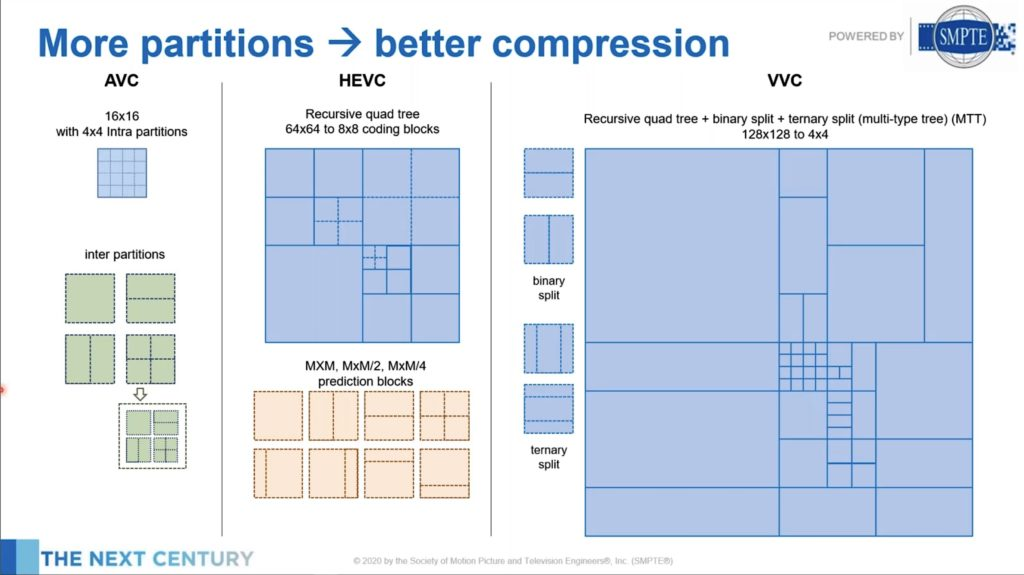
\includegraphics[width=0.9\textwidth]{CTUs}}
\end{center}

\section*{VVC vs HEVC vs AVC}
\begin{center}
  \href{https://www.linkedin.com/pulse/video-coding-standards-comparison-sraas}{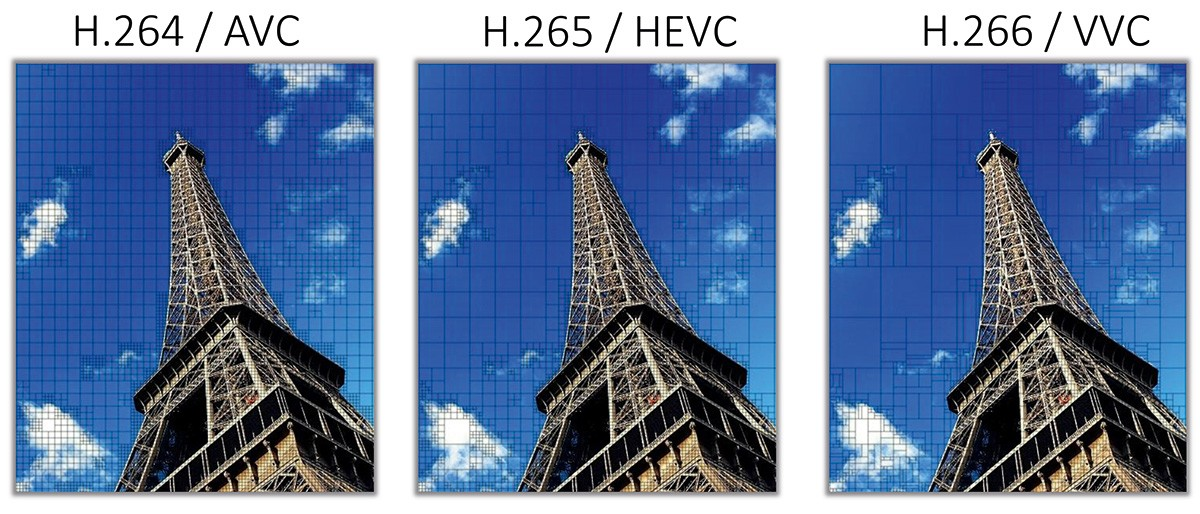
\includegraphics[width=\textwidth]{AVC_HEVC_VVC}}
\end{center}
